\documentclass[a4paper,12pt]{article}
\usepackage[utf8]{inputenc}
\usepackage{polski}
\usepackage{graphicx}
\usepackage[lmargin=2cm,rmargin=2cm]{geometry}
\title{Najdłuższy cykl prosty w grafie}
\author{Kamil Chlebek, Arkadiusz Błasiak, Piotr Jaromin}
\begin{document}
\maketitle
\newpage
\tableofcontents
\newpage
\section{Teoria}
\subsection{Graf}

\textbf{Graf} to zbiór wierzchołków, które mogą być połączone krawędziami w taki sposób, że każda krawędź kończy się i zaczyna w którymś z wierzchołków

\begin{figure}[htbp]
\center{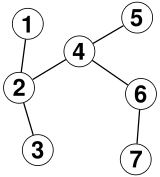
\includegraphics[scale=0.8]{grafnieskierowany.png}}
\caption{Graf nieskierowany}
\end{figure}
\subsection{Cykl}
\textbf{Cykl} jest ścieżką, która rozpoczyna się i kończy w tym samym wierzchołku (ścieżka ta może posiadać wielokrotnie ten sam wierzchołek). Cykl o długości 1 nazywa się pętlą.
\\
\\
\textbf{Cykl prosty} - jest ścieżką, która rozpoczyna się i kończy w tym samym wierzchołku (ścieżka ta nie może posiadać wielokrotnie tego samego wierzchołka)
\begin{figure}[htbp]
\center{
\includegraphics[scale=0.078]{hamilton.png}}
\caption{Cykl prosty w grafie}
\end{figure}
\subsection{Algorytm genetyczny}
\textbf{Algorytm genetyczny} - rodzaj algorytmu przeszukującego przestrzeń alternatywnych rozwiązań problemu w celu wyszukania rozwiązań najlepszych.
\subsubsection{Etapy algorytmu}
\begin{enumerate}
\item Losowanie początkowej populacji
\item Selekcja - populacja jest poddawana ocenie (korzystając z funkcji oceny), wybierane są najlepsze osobniki
\item Krzyżowanie - złączanie uprzednio wybranych osobników
\item Mutacja - wprowadzenie losowych zmian w osobniku
\item Rodzi się kolejne pokolenie. Najlepsze osobniki są powielane, a najsłabsze usuwane. Jeżeli nie znaleziono dostatecznie dobrego rozwiązania, algorytm powraca do kroku drugiego. W przeciwnym wypadku wybieramy najlepszego osobnika z populacji.
\end{enumerate}
\subsubsection{Funkcja oceny}
Funkcja oceny to miara jakości dowolnego osobnika w populacji. Dla każdego osobnika jest ona obliczana na podstawie sumy odległości między wierzchołkami.
\\
Dla dwóch wierzchołków: $\sqrt[]{(v2x-v1x)^{2} + (v2y-v1y)^{2}}$
\subsubsection{Krzyżowanie}
Krzyżowanie zachodzi z pewnym prawdopodobieństwem.
\\
Pierwsza połowa chromosomów z jednego osobnika jest łączona z drugą połową drugiego osobnika oraz druga połowa pierwszego z pierwszą połową drugiego. Wynikiem są dwa nowe osobniki. 
\begin{figure}[htbp]
\center{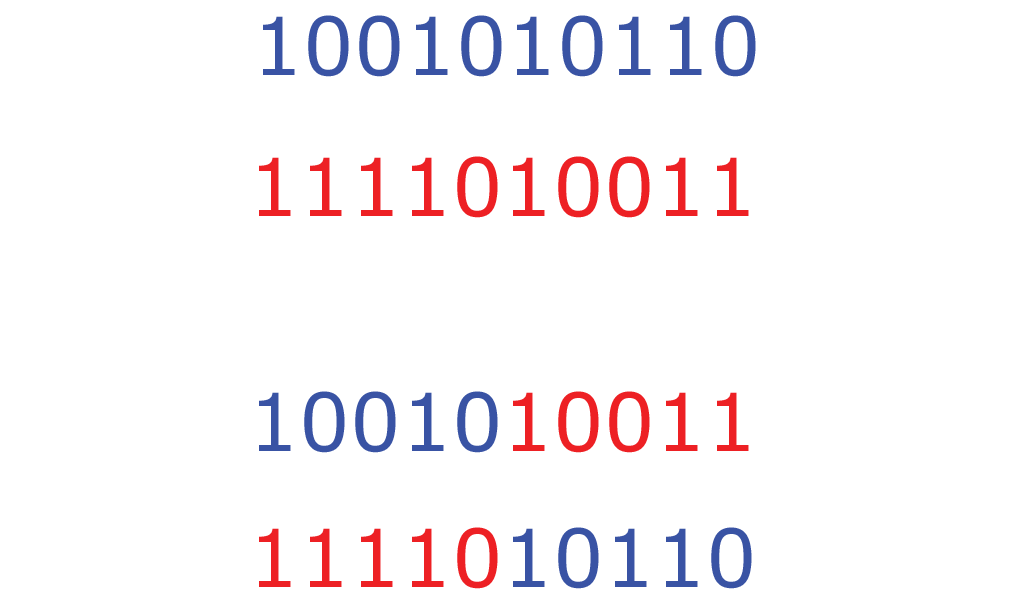
\includegraphics[scale=0.20]{krzyz.png}}
\caption{Krzyżowanie}
\end{figure}
\subsubsection{Mutacja}
TODO
\end{document}